\chapter{Results and Discussion}
\label{chp:results_and_discussion}

\lettrine{O}{utcomes} of the simulation cases are presented. The performance of the guidance law is assessed based on performance in the numerical experiments. Consideration of the methodology is used to explain some of the observed behaviours, and deficiencies are noted for improvement.

\section{Baseline Case Runs}
The baseline trajectory cases outlined in Tables \ref{tab:trajectory_cases} and \ref{tab:trajectory_case_params} were simulated, and the main results are shown in Table \ref{tab:outputs_1_summary}.
\begin{table}[H]
    \centering
    \begin{tabular}{lR{3cm}R{2.5cm}rr}
        \toprule
        \textbf{Case ID} & Convergence Tolerance & Time of Flight (d) & \# Revolutions & CPU Time (s) \\
        \midrule
        A                & 0.001                 & 621                & 862            & 17.6         \\
        B                & 0.03                  & 498                & 501            & 16.9         \\
        C                & 0.005                 & 802                & 1560           & 38.3         \\
        D                & 0.005                 & 63                 & 62             & 10.1         \\
        \bottomrule
    \end{tabular}
    \caption{Summary of outcomes for each case.}
    \label{tab:outputs_1_summary}
\end{table}

Case-by-case plots of the time history of the orbital elements and trajectories are shown in the proceeding sections.
\subsection{Plots: Cases A-D}
\begin{figure}[H]
    \centering
    \begin{subfigure}[t]{0.4\textwidth}
        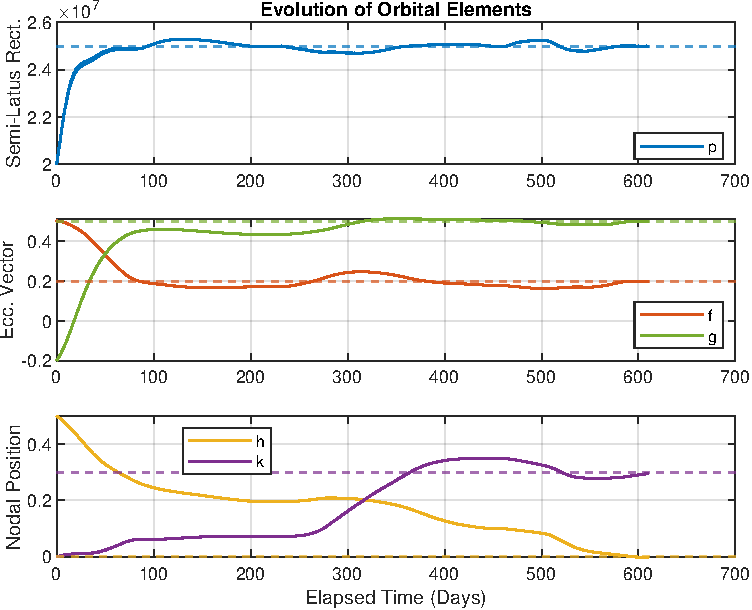
\includegraphics[width=\textwidth]{figures/benchmark_transfer/orbital_elements.pdf}
        \caption{Evolution of orbit elements in time.}
        \label{fig:results_a_a}
    \end{subfigure}
    \begin{subfigure}[t]{0.59\textwidth}
        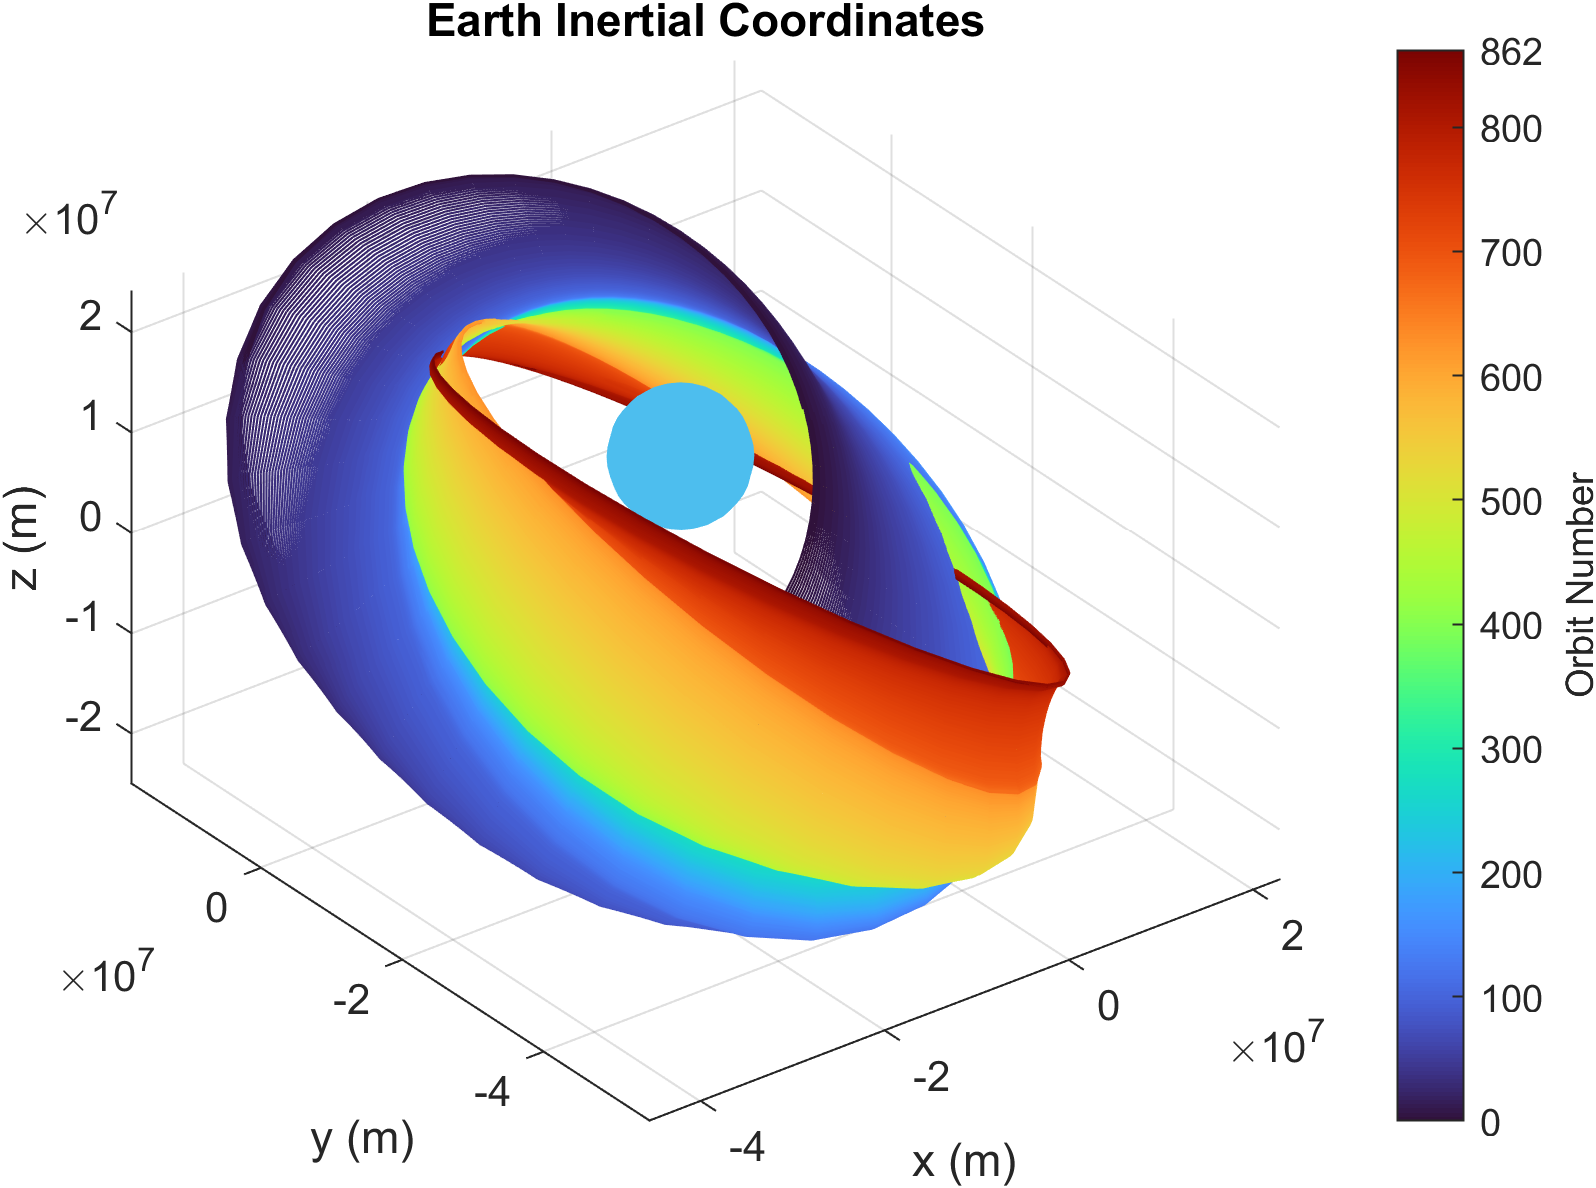
\includegraphics[width=\textwidth]{figures/benchmark_transfer/trajectory_plot.png}
        \caption{Trajectory plot.}
        \label{fig:results_a_b}
    \end{subfigure}
    \caption{Orbital elements and trajectory for case A.}
    \label{fig:results_a}
\end{figure}
\begin{figure}[H]
    \centering
    \begin{subfigure}[t]{0.4\textwidth}
        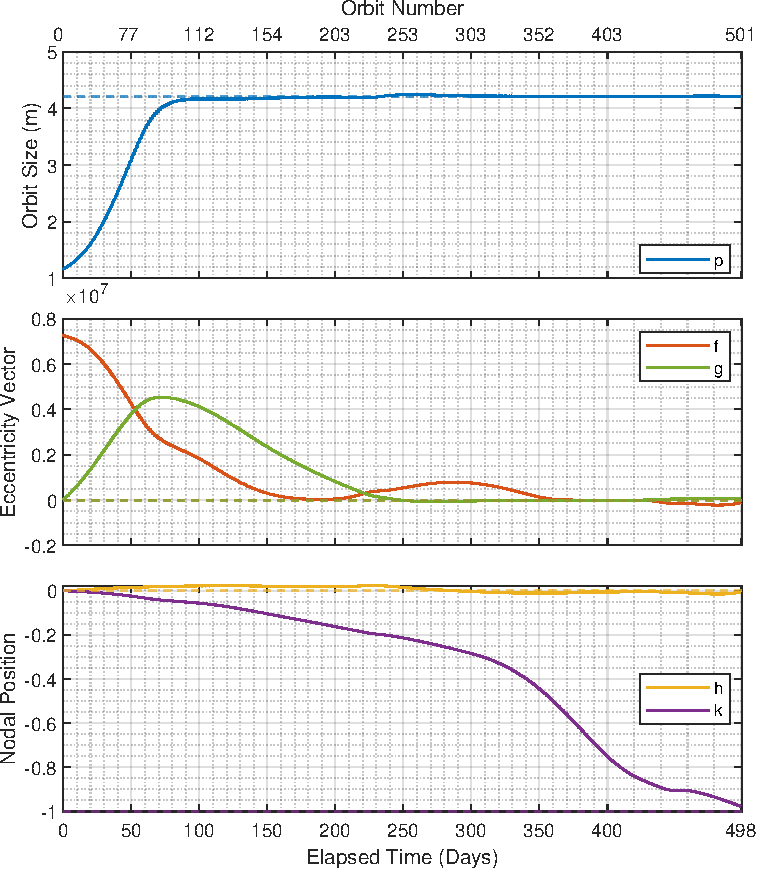
\includegraphics[width=\textwidth]{figures/oguri_G/orbital_elements.pdf}
        \caption{Evolution of orbit elements in time.}
        \label{fig:results_results_b_a}
    \end{subfigure}
    \begin{subfigure}[t]{0.59\textwidth}
        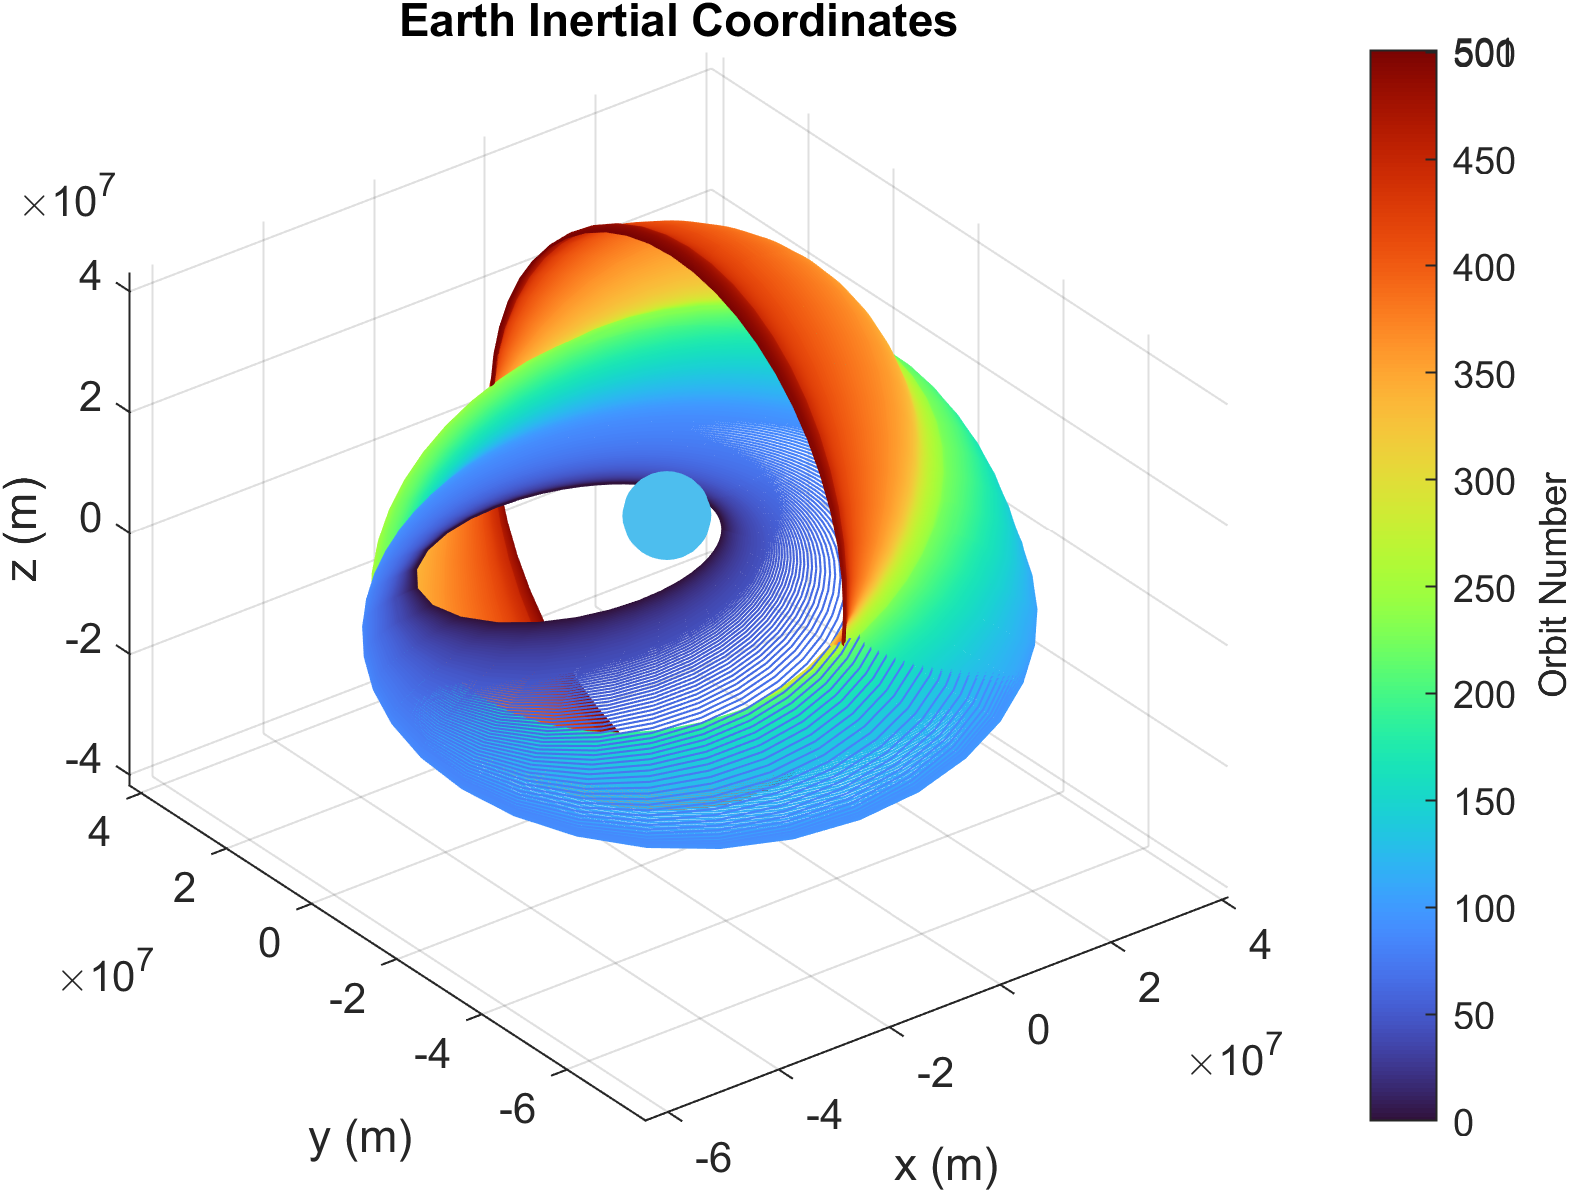
\includegraphics[width=\textwidth]{figures/oguri_G/trajectory_plot.png}
        \caption{Trajectory plot.}
        \label{fig:results_results_b_b}
    \end{subfigure}
    \caption{Orbital elements and trajectory for case B.}
    \label{fig:results_results_b}
\end{figure}
\begin{figure}[H]
    \centering
    \begin{subfigure}[t]{0.4\textwidth}
        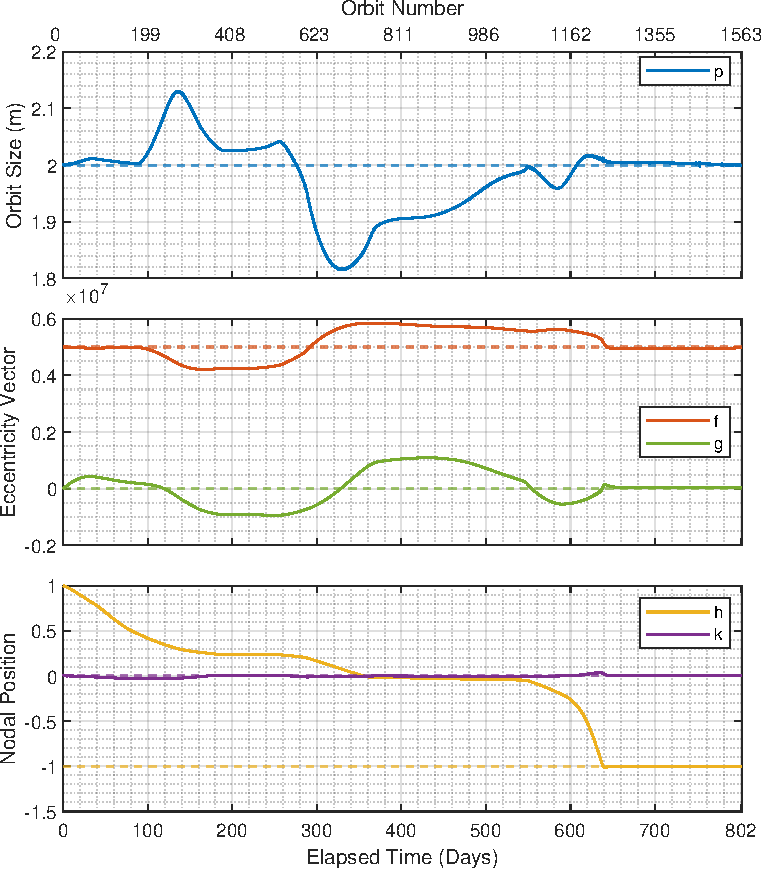
\includegraphics[width=\textwidth]{figures/plane_change/orbital_elements.pdf}
        \caption{Evolution of orbit elements in time.}
        \label{fig:results_c_a}
    \end{subfigure}
    \begin{subfigure}[t]{0.59\textwidth}
        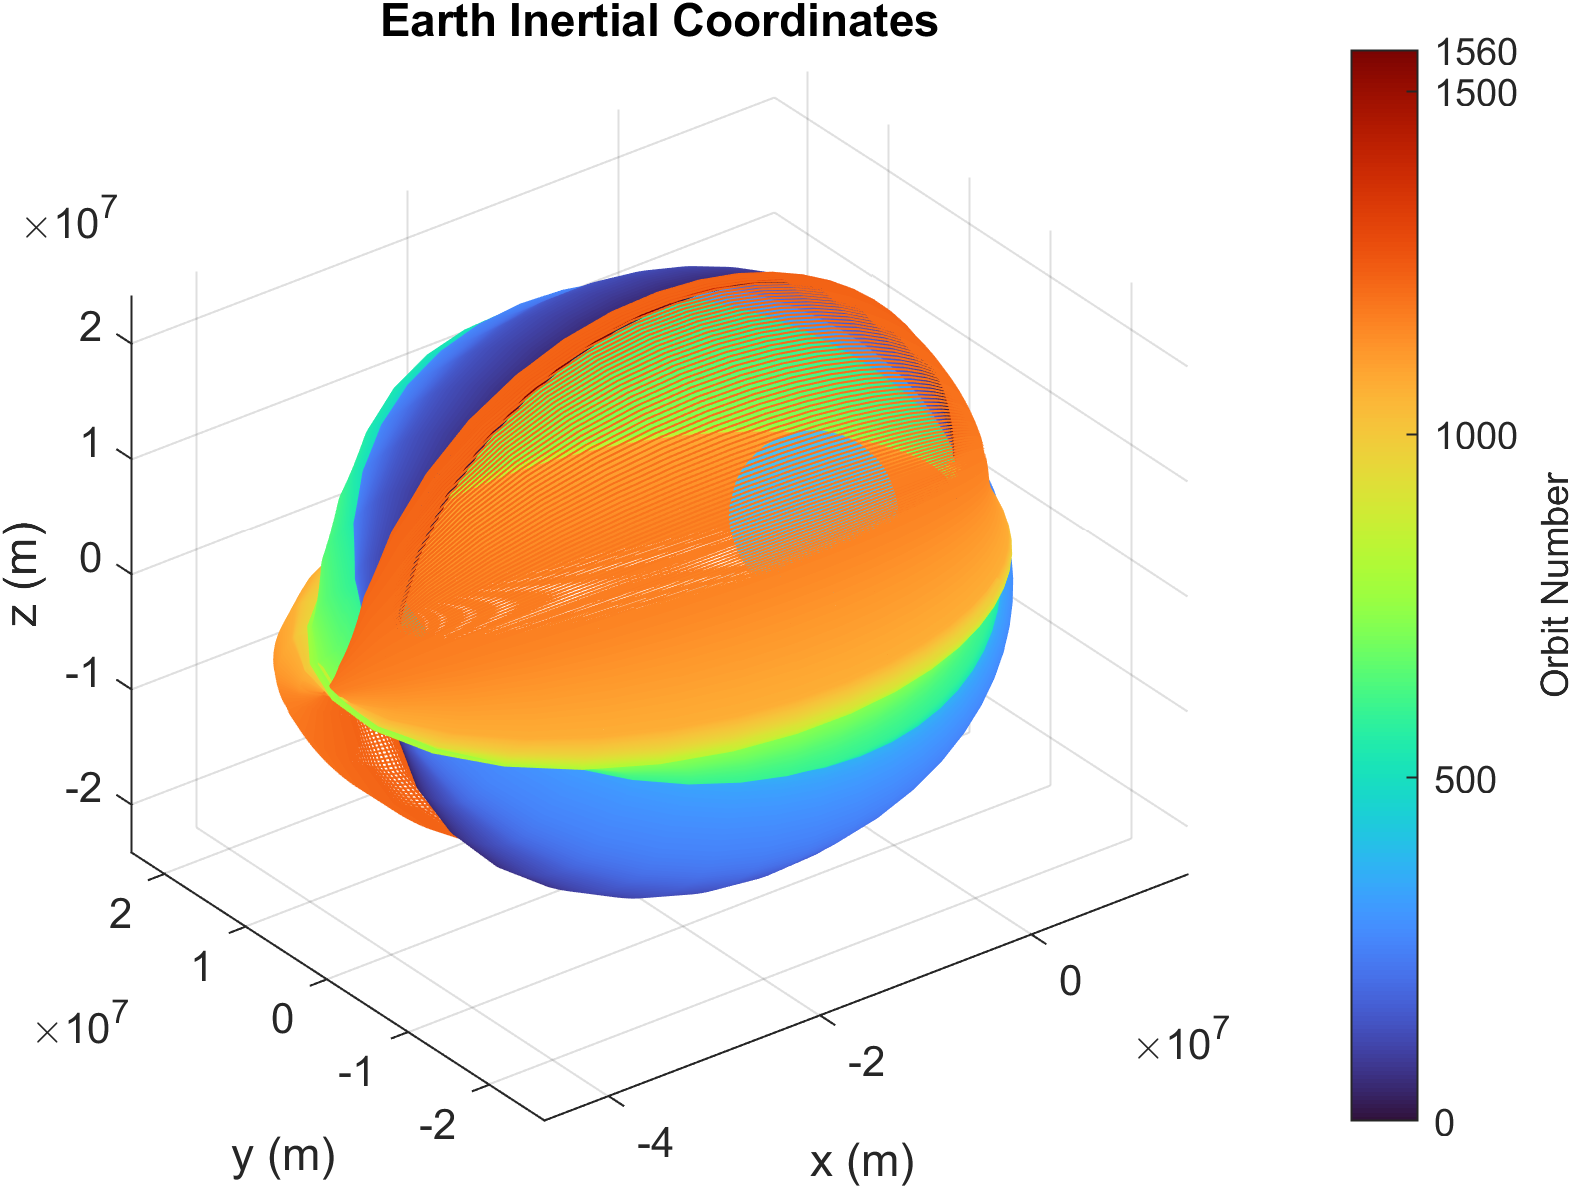
\includegraphics[width=\textwidth]{figures/plane_change/trajectory_plot.png}
        \caption{Trajectory plot.}
        \label{fig:results_c_b}
    \end{subfigure}
    \caption{Orbital elements and trajectory for case C.}
    \label{fig:results_c}
\end{figure}

\begin{figure}[H]
    \centering
    \begin{subfigure}[t]{0.4\textwidth}
        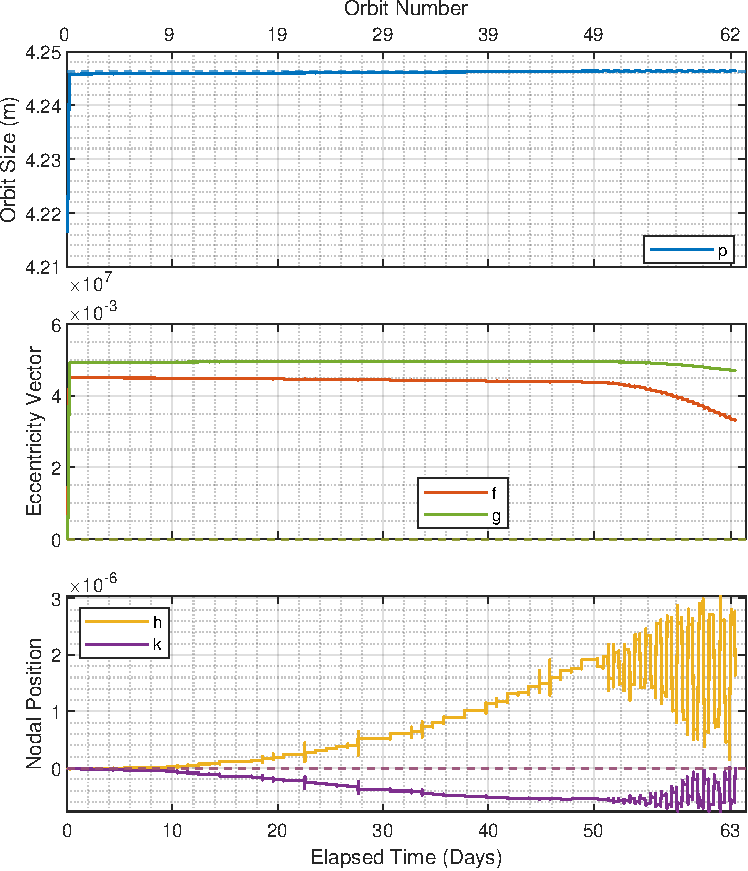
\includegraphics[width=\textwidth]{figures/geo_disposal/orbital_elements.pdf}
        \caption{Evolution of orbit elements in time.}
        \label{fig:results_results_c_a}
    \end{subfigure}
    \begin{subfigure}[t]{0.59\textwidth}
        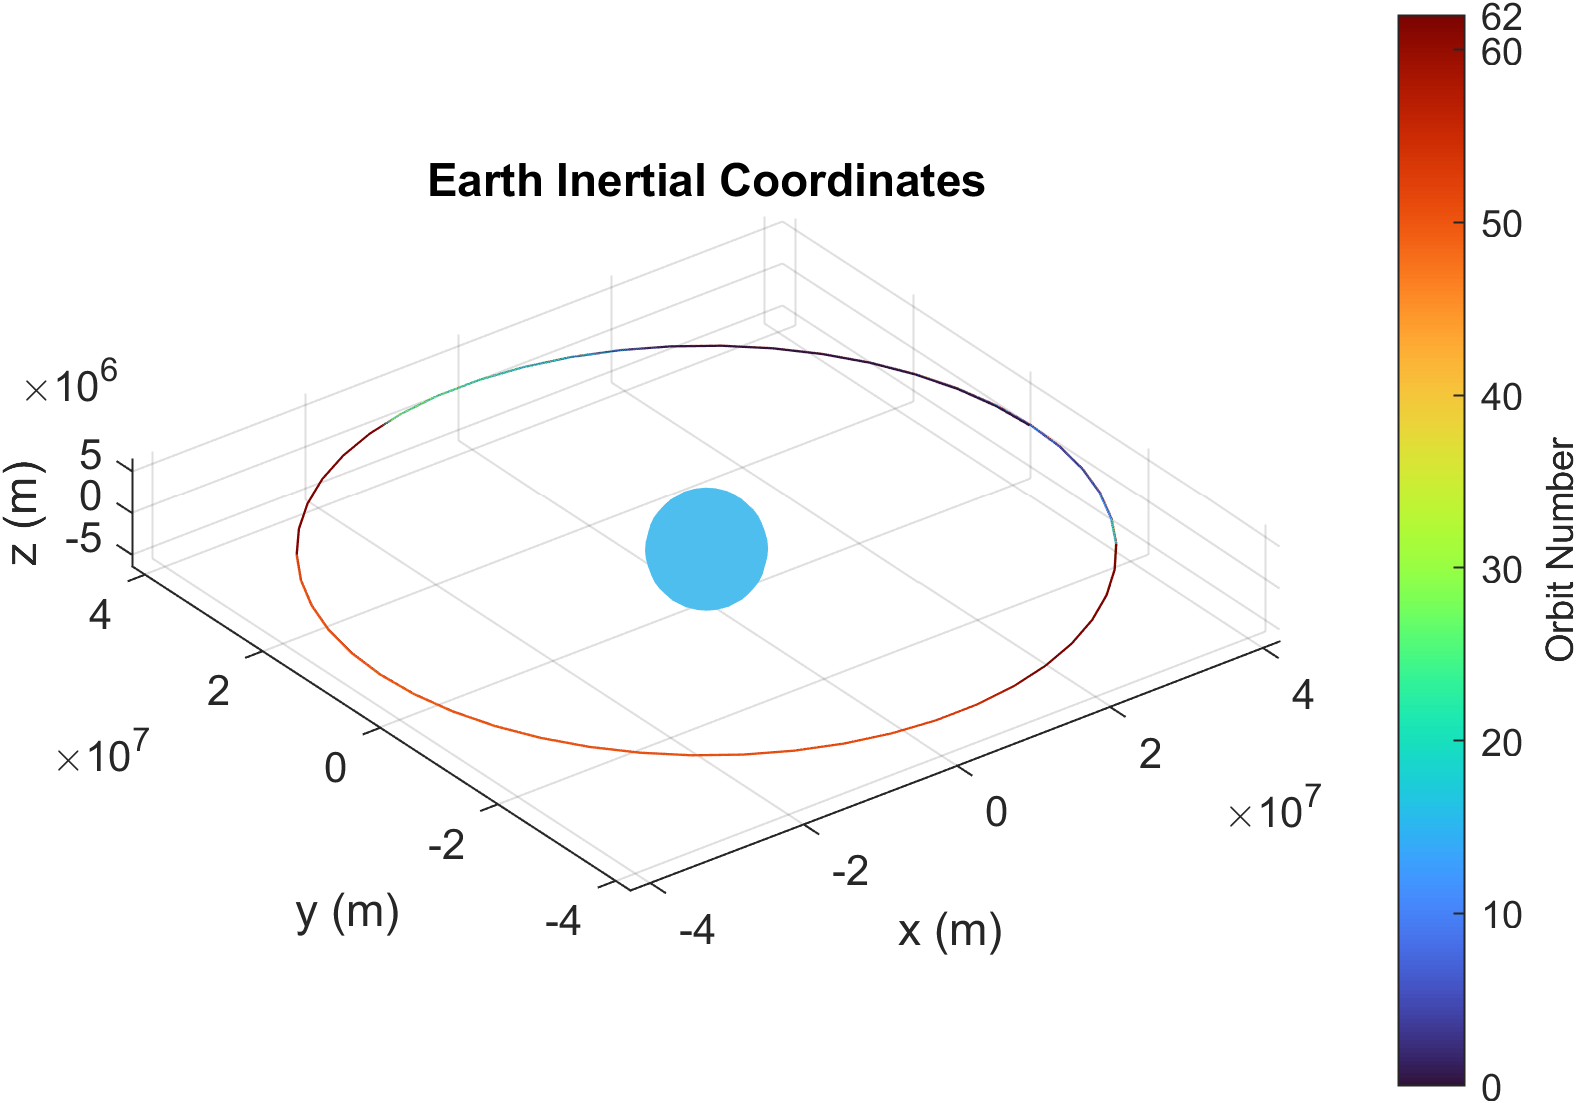
\includegraphics[width=\textwidth]{figures/geo_disposal/trajectory_plot.png}
        \caption{Trajectory plot.}
        \label{fig:results_results_c_b}
    \end{subfigure}
    \caption{Orbital elements and trajectory for case D.}
    \label{fig:results_results_c}
\end{figure}

\newpage
The ``banding'' of colours in the trajectory plots highlight the tendency of the guidance law to segment the trajectory into distinguishable phases rather than a smooth continuous maneuver. This can be attributed to the properties of the guidance law discussed in Section \ref{sec:quail_properties}. Additionally, the tendency of the guidance law to continue changing orbital elements even after reaching their target values shows the relaxation of Lyapunov stability.

For case C, as speculated in the previous section, the guidance law does not smoothly vary the orbit. The direction of applied thrust varies by \ang{180} over the course of the maneuver, and the Sun is not always in a suitable position for thrust production. Hence, even though the semilatus rectum (\(p\)) is supposed to remain constant, it actually varies so that some of the other orbital elements become easier to change. In effect, the guidance law has instated its own ``intermediate orbit''.

Case D highlights a significant issue with the guidance law: it is extremely slow to finish off ``the last mile''. Note that all of the cases were run with convergence tolerances exceeding \(0.001\) -- this was done because smaller tolerances were either not achievable or took excessive numbers of orbits to converge.

This issue with last mile convergence may be attributed to the cone angle adaptation heuristic; not producing thrust exactly in the direction needed by the Q-Law incurs a sort of steady-state error similar to that in a proportional feedback controller.

\subsection{Animations: Cases A-C}
Animations of the trajectories in cases A-C are shown in the proceeding figures (case D is excluded because the change in shape is negligible). Seeing the trajectories animated in 3D space may help provide a more comprehensible view of what the guidance law is doing. Note that the 3D camera is rotated compared to the plots in the previous section.

Note: a JavaScript-enabled PDF viewer (e.g. Adobe Reader, Foxit Reader) is required for playing the animations.

Each animation plays at 10 frames per second by default, with approximately 50 frames of animation per case.

\begin{figure}[H]
    \animategraphics[width=\textwidth, controls, loop]{10}{animations/benchmark_transfer/anim-}{1}{50}
    \caption{Trajectory animation for case A.}
    \label{fig:anim_a}
\end{figure}
The segmentation of the trajectory is much easier to see in animation form. There are obvious points in the trajectory where the orbit ``pauses'', waiting for the Sun to move into a better position. This includes the time spent feathering the solar sail.

It is reasonable to conclude that time spent waiting for the Sun is essentially waste, and there may exist a better trajectory which spends less time paused.
\begin{figure}[H]
    \animategraphics[width=\textwidth, controls, loop]{10}{animations/oguri_case_G/anim-}{1}{47}
    \caption{Trajectory animation for case B.}
    \label{fig:anim_b}
\end{figure}

This trajectory is flown much more smoothly than in case A, but there is some stalling near the end.

\begin{figure}[H]
    \animategraphics[width=\textwidth, controls, loop]{10}{animations/plane_change/anim-}{1}{50}
    \caption{Trajectory animation for case C.}
    \label{fig:anim_c}
\end{figure}
Trajectory segmentation is most evident in this animation.

Overall, it is impressive that the guidance law is convergent in all of the test cases. However, it is far from perfect. Most notably, it is extremely slow at advancing the orbit in certain segments. Hence, the first extended study aims to search for trajectories with lower time of flight through tuning the guidance weight \(W_{\moe}\).

Tuning the weights of the Q-Law is equivalent to changing the ``greediness strategy'' of the local optimization being done at each timestep; the baseline Q-Law always attempts to maximize \(-\dot{Q}\) (in a greedy fashion), and adjusting \(W_{\moe}\) helps ``steer the greediest direction'' at one timestep to help the guidance law at a later timestep. There may exist a \textbf{local strategy} which can set up a better trajectory at a \textbf{global level}.


\newpage
\section{Time of Flight Optimization Study}
Global weight optimization was performed for the first two baseline cases. The optimized guidance law tunings are compared against their unoptimized counterparts in Table \ref{tab:outputs_2_summary}.

\begin{table}[H]
    \centering
    \begin{tabular}{L{5cm}L{2.5cm}L{2.5cm}L{3cm}}
        \toprule
        \textbf{Case}                          & Time of Flight (d) & Number of Revolutions & \(\Delta v\) Expenditure (m/s) \\
        \midrule
        A, Baseline                            & 621                & 862                   & 6459.6                         \\
        \rowcolor{green!20!white}A, Optimized  & 385                & 680                   & 6216.1                         \\
        B, Baseline                            & 498                & 501                   & 9640.5                         \\
        \rowcolor{green!20!white} B, Optimized & 377                & 326                   & 8315.4                         \\
        \bottomrule
    \end{tabular}
    \caption{Comparison of optimized cases against their baselines.}
    \label{tab:outputs_2_summary}
\end{table}

The two cases still use their original convergence tolerances in the optimized tunings.

The improvement in time-of-flight (and number of revolutions) is remarkable. By inspecting the plots of the orbital elements in the proceeding section, it is clear that adjusting \(W_\moe\) changes the ``strategy'' employed by the guidance law.

One important note is that the stochastic optimization runs do not guarantee the discovery of a global minimum; the weights corresponding to the absolute lowest time of flight found over all optimization runs were used for the cases shown in the proceeding sections, but there may exist a solution with a lower time of flight that was not discovered. However, this is likely not a great issue; several different combinations of \(W_\moe\) all yielding a reduction in time of flight were found, and many solutions had a time of flight value within about 1\% of the absolute minimum found in the optimization runs. It is highly unlikely then that a dramatically lower time of flight could have been found even with more compute time.

This highlights a great weakness of the approach taken by QUAIL -- since there is so little that can be said about the guidance law analytically, it is very difficult to make any performance assertions about the global trajectory.

Another important point to make is that QUAIL requires fine tuning to achieve shorter time of flight. While it can work out of the box, it needs to be adjusted for each mission to fly trajectories more efficiently. This is much like how classical feedback control laws are tuned to match a certain control problem.

\newpage
\subsection{Plots}
\label{sec:bench_case_plot}
Baseline \(W_{\moe}\): \(\{1, 1, 1, 1, 1\}\)


Optimal \(W_{\moe}\): \(\{1.774, 0.5149, 0.3327, 9.925, 0.5317\}\)

\begin{figure}[H]
    \centering
    \begin{subfigure}[t]{0.49\textwidth}
        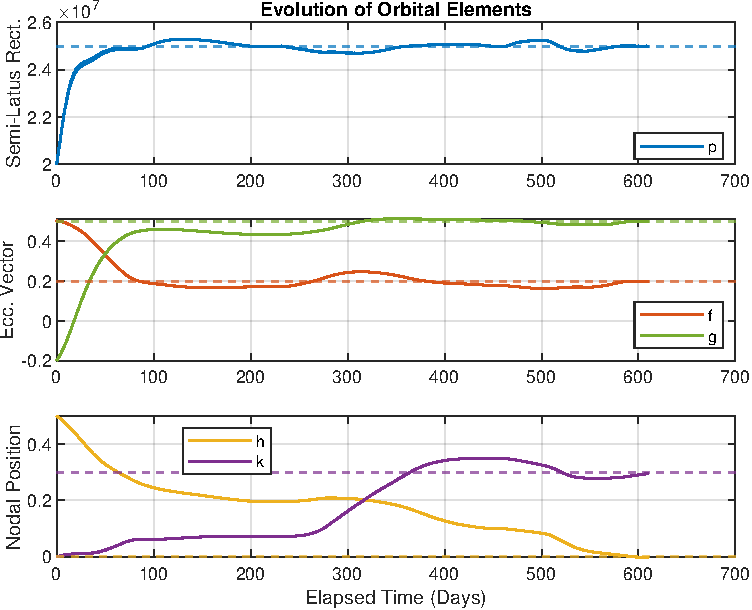
\includegraphics[width=\textwidth]{figures/benchmark_transfer/orbital_elements.pdf}
        \caption{Baseline.}
        \label{fig:results_optim_a_1}
    \end{subfigure}
    \begin{subfigure}[t]{0.49\textwidth}
        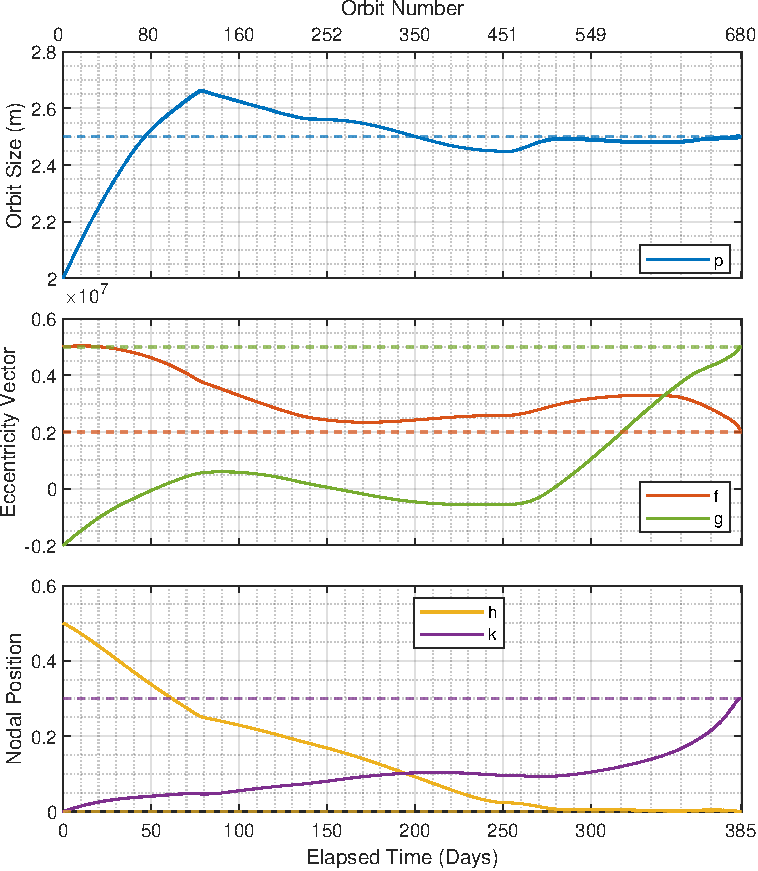
\includegraphics[width=\textwidth]{figures/benchmark_optim/orbital_elements.pdf}
        \caption{Optimized.}
        \label{fig:results_optim_a_2}
    \end{subfigure}
    \caption{Case A, orbital elements.}
    \label{fig:results_optim_a}
\end{figure}

\begin{figure}[H]
    \centering
    \begin{subfigure}[t]{0.49\textwidth}
        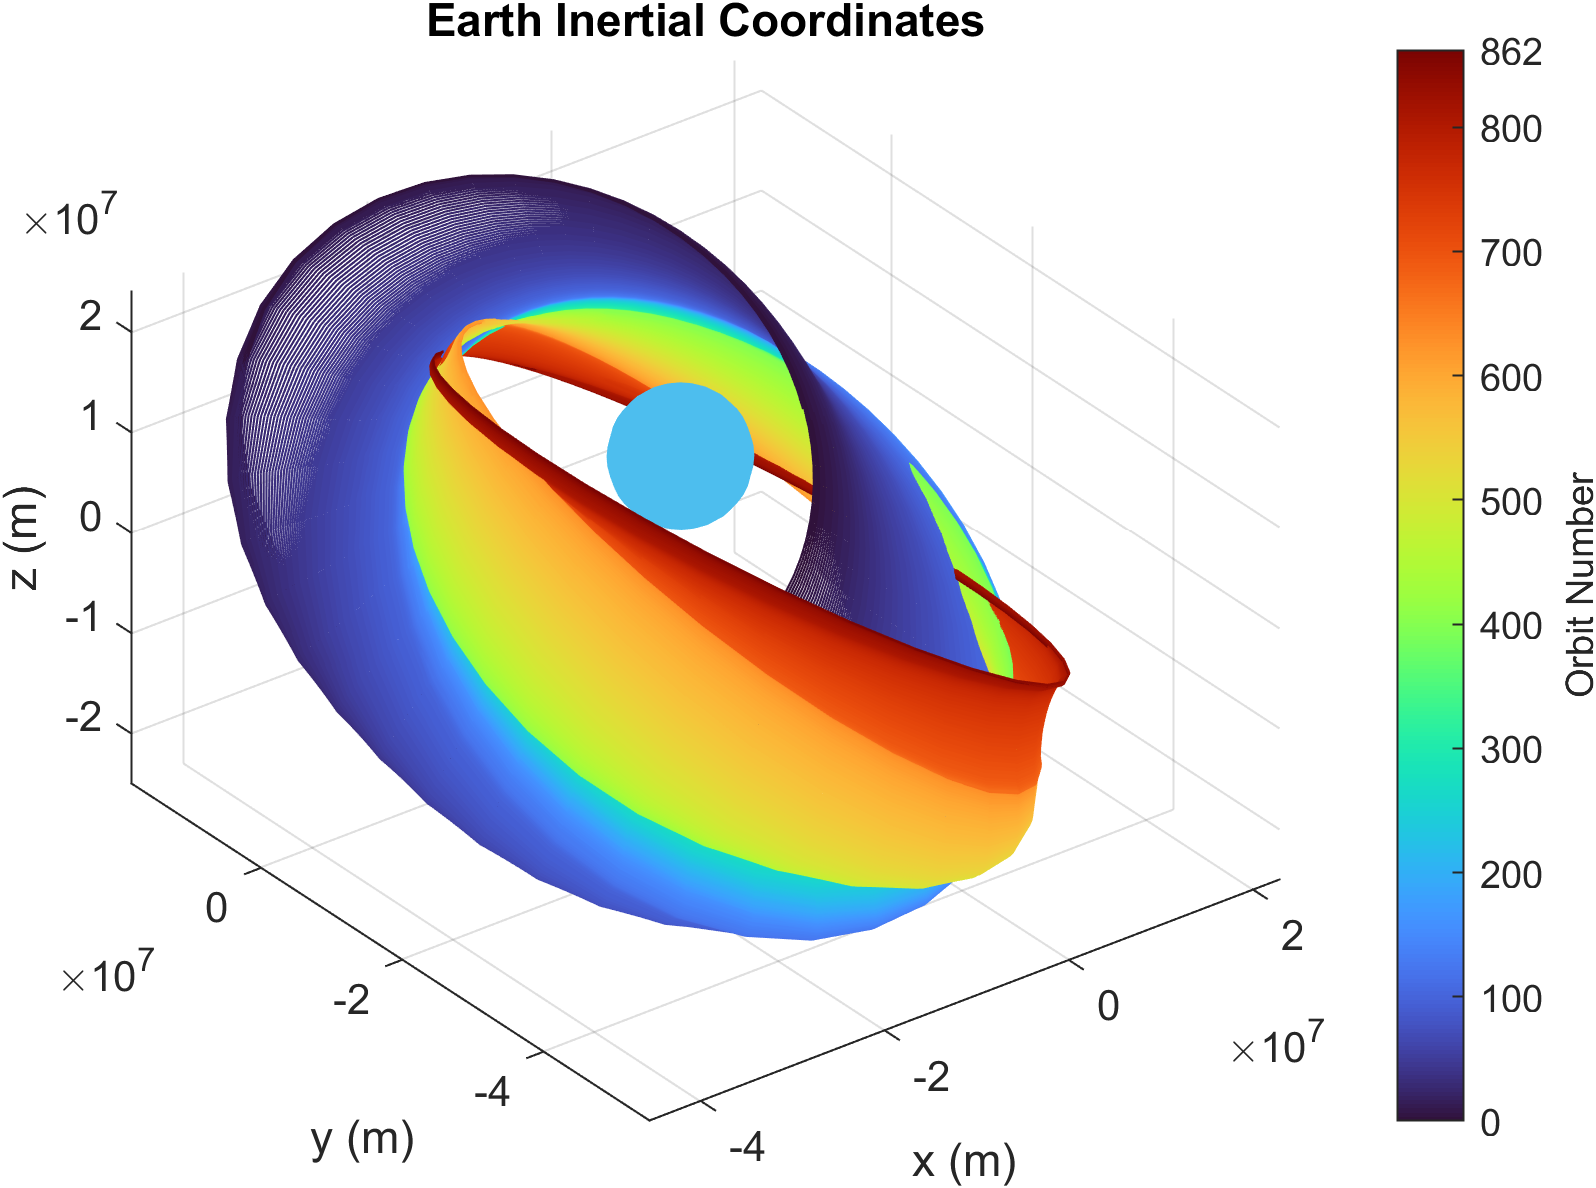
\includegraphics[width=\textwidth]{figures/benchmark_transfer/trajectory_plot.png}
        \caption{Baseline.}
        \label{fig:results_traj_optim_a_1}
    \end{subfigure}
    \begin{subfigure}[t]{0.49\textwidth}
        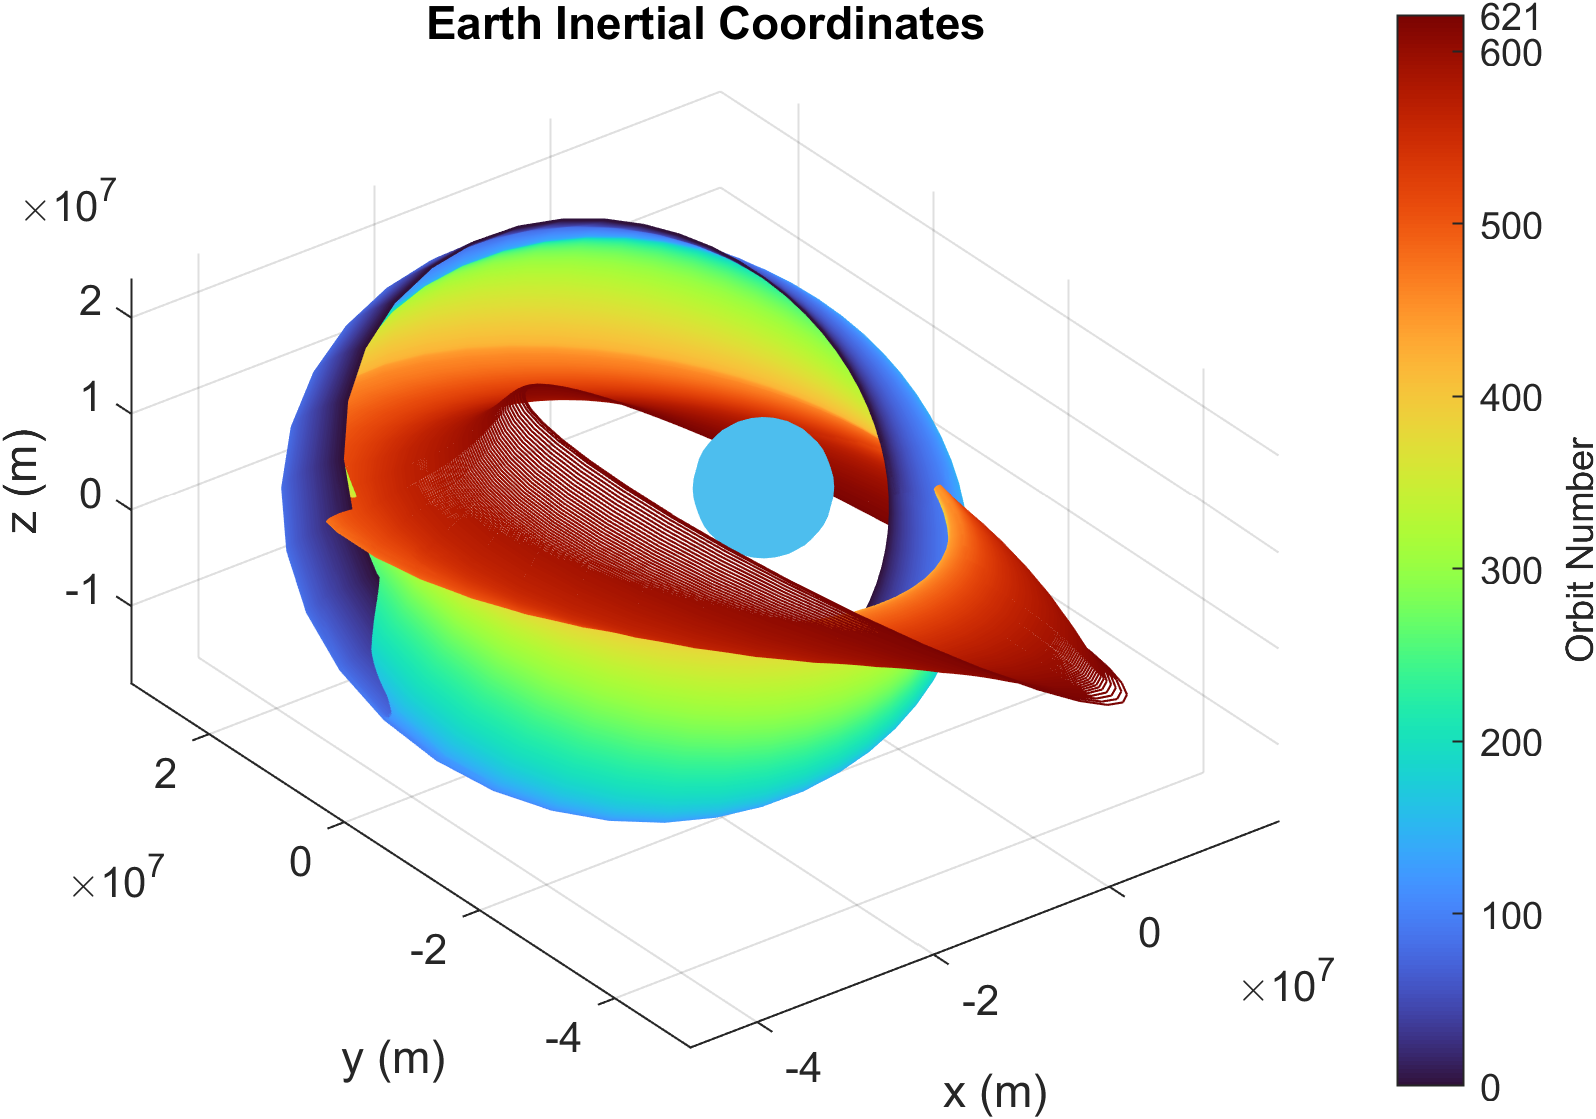
\includegraphics[width=\textwidth]{figures/benchmark_optim/trajectory_plot.png}
        \caption{Optimized.}
        \label{fig:results_traj_optim_a_2}
    \end{subfigure}
    \caption{Case A, trajectory plot.}
    \label{fig:results_traj_optim_a}
\end{figure}


\newpage
\subsection{Case B}
\label{sec:gso_case_plot}
Baseline \(W_{\moe}\): \(\{1, 1, 1, 1, 1\}\)

Optimal \(W_{\moe}\): \(\{5.688, 1.178, 1.434, 3.545, 5.568\}\)

\begin{figure}[H]
    \centering
    \begin{subfigure}[t]{0.49\textwidth}
        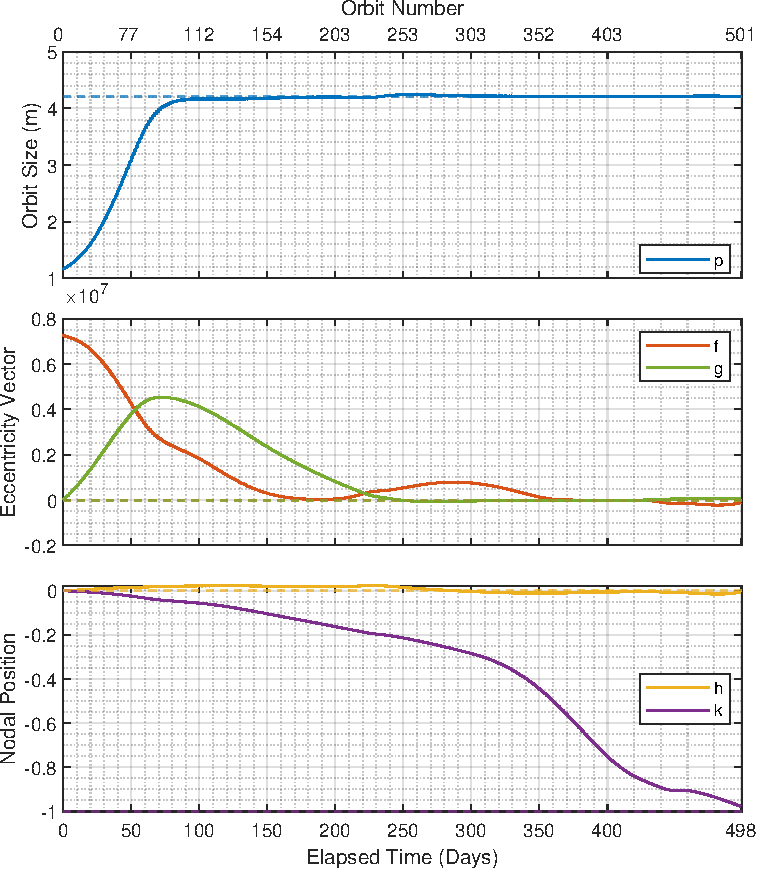
\includegraphics[width=\textwidth]{figures/oguri_G/orbital_elements.pdf}
        \caption{Baseline.}
        \label{fig:results_optim_b_1}
    \end{subfigure}
    \begin{subfigure}[t]{0.49\textwidth}
        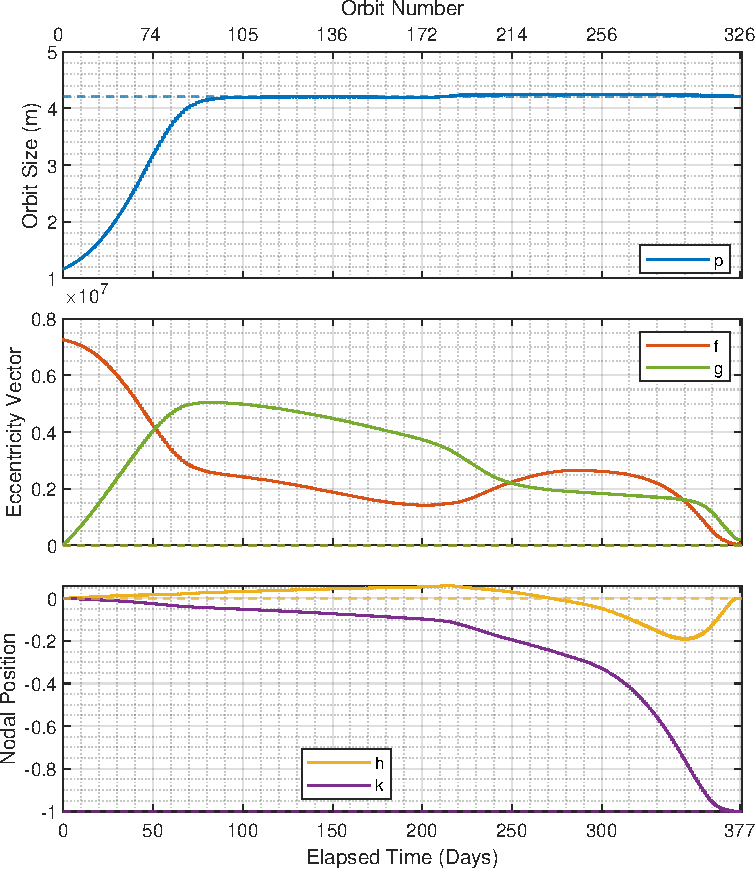
\includegraphics[width=\textwidth]{figures/oguri_optim/orbital_elements.pdf}
        \caption{Optimized.}
        \label{fig:results_optim_b_2}
    \end{subfigure}
    \caption{Case B, orbital elements.}
    \label{fig:results_optim_b}
\end{figure}

\begin{figure}[H]
    \centering
    \begin{subfigure}[t]{0.49\textwidth}
        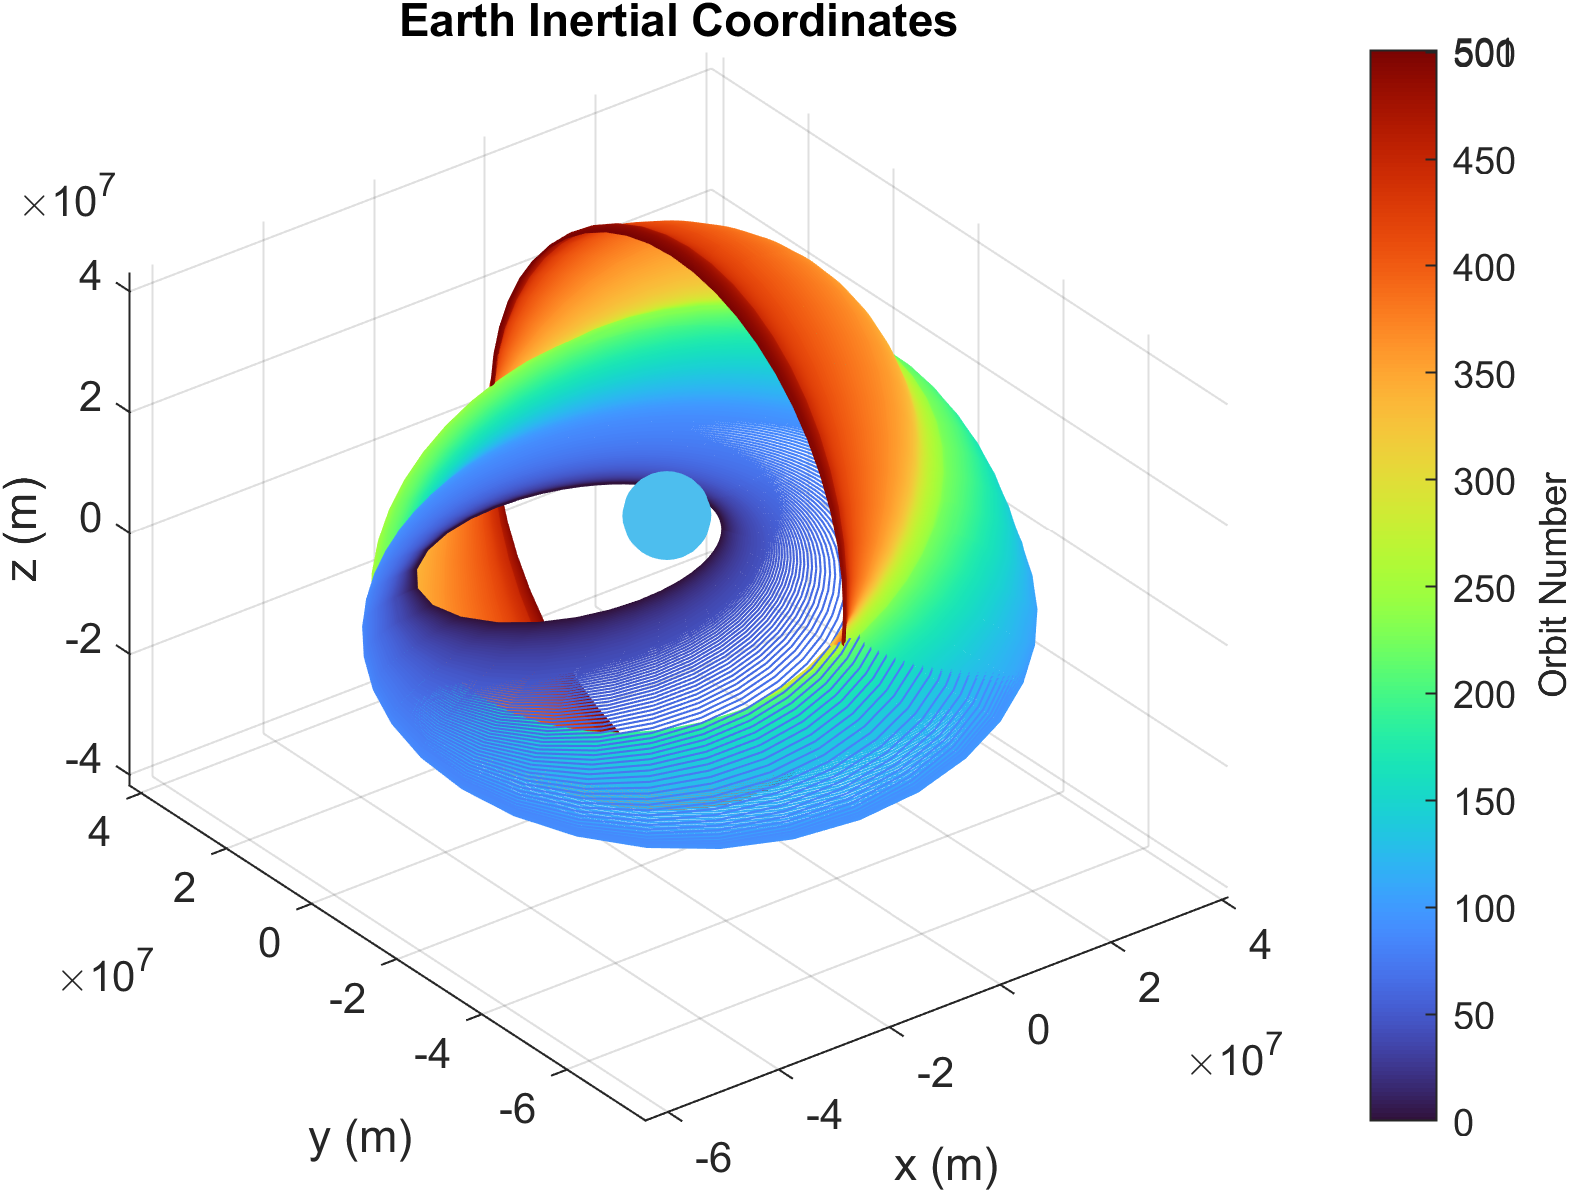
\includegraphics[width=\textwidth]{figures/oguri_G/trajectory_plot.png}
        \caption{Baseline.}
        \label{fig:results_traj_optim_b_1}
    \end{subfigure}
    \begin{subfigure}[t]{0.49\textwidth}
        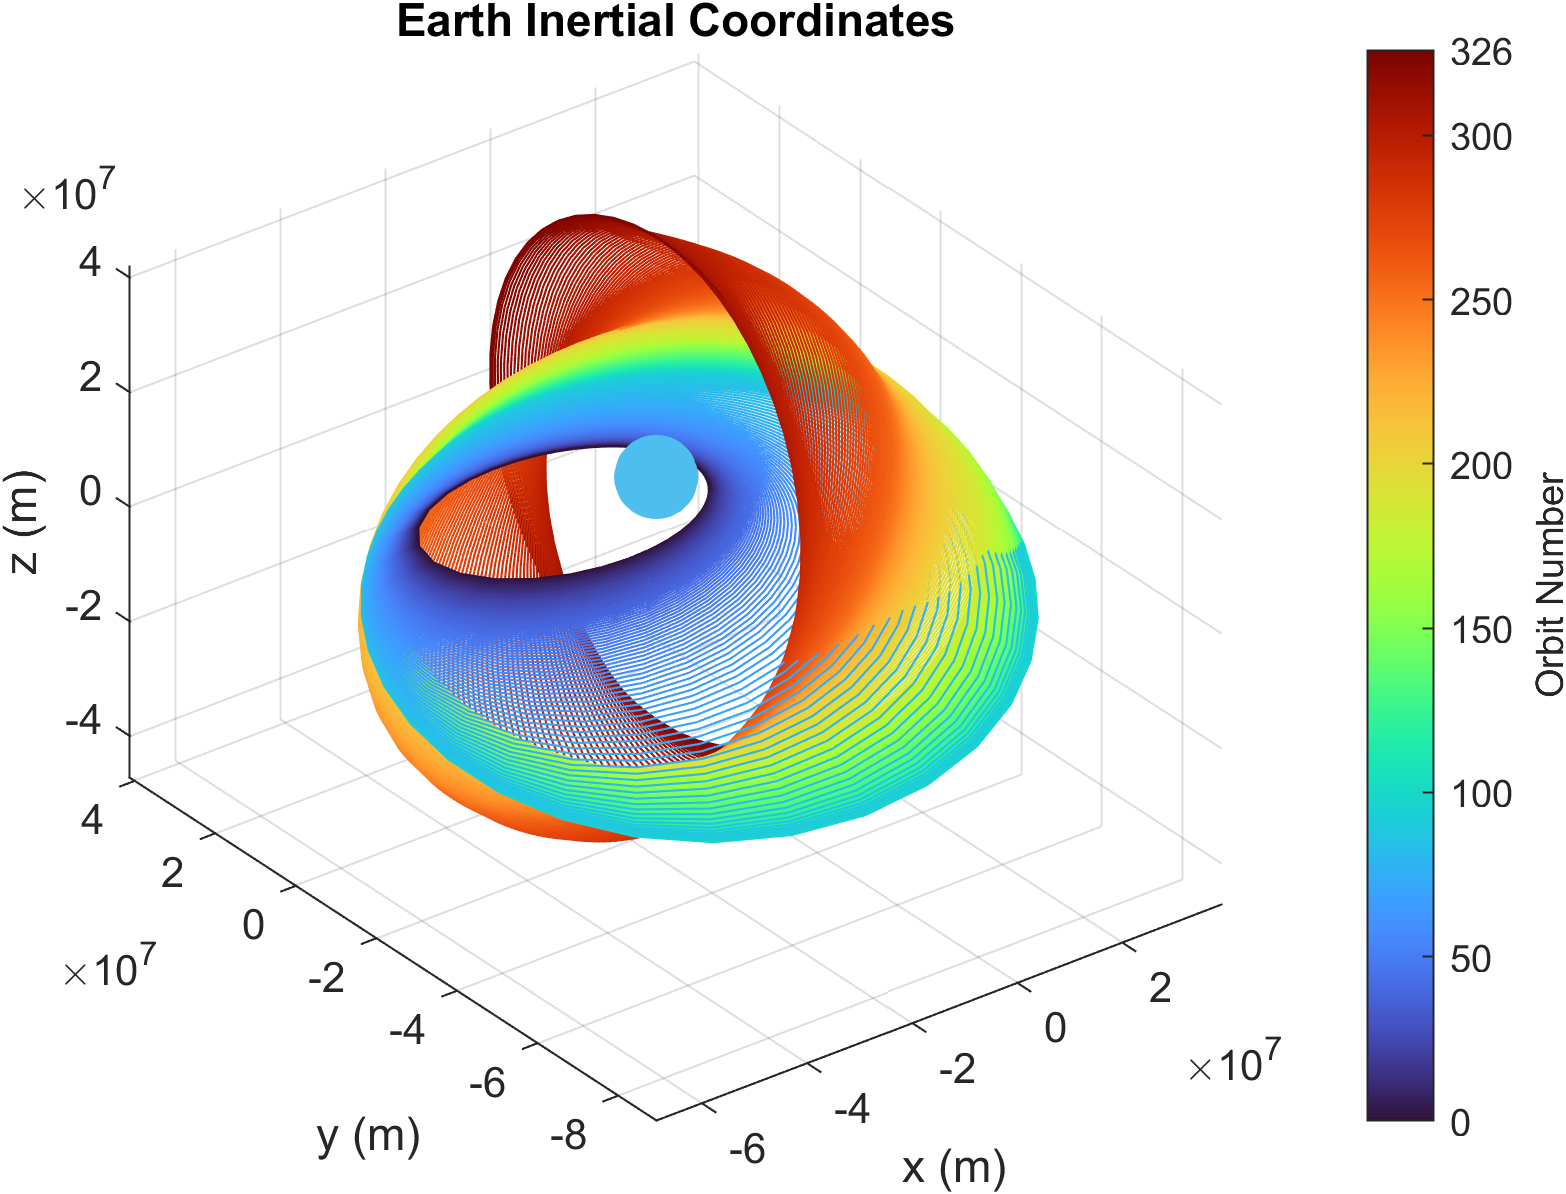
\includegraphics[width=\textwidth]{figures/oguri_optim/trajectory_plot.png}
        \caption{Optimized.}
        \label{fig:results_traj_optim_b_2}
    \end{subfigure}
    \caption{Case B, trajectory plot.}
    \label{fig:results_traj_optim_b}
\end{figure}

\subsection{Animations}
\begin{figure}[H]
    \begin{animateinline}[controls,width=\linewidth, loop]{10}
        \multiframe{50}{i=1+1}{
            \includegraphics[height=0.5\textwidth]{animations/benchmark_transfer/anim-\i}%
            \includegraphics[height=0.5\textwidth]{animations/benchmark_transfer_optim/anim-\i}}
    \end{animateinline}
    \caption{Case A before/after optimization.}
    \label{fig:benchmark_optim_anim}
\end{figure}
% View: -70, 20
\begin{figure}[H]
    \begin{animateinline}[controls,width=\linewidth, loop]{10}
        \multiframe{47}{i=1+1}{
            \includegraphics[height=0.5\textwidth]{animations/oguri_case_G/anim-\i}%
            \includegraphics[height=0.5\textwidth]{animations/oguri_case_G_optim/anim-\i}}
    \end{animateinline}
    \caption{Case B before/after optimization.}
    \label{fig:g_optim_anim}
\end{figure}

By emphasizing certain elements over others, the guidance law is more willing to accept an increase in error in one element for a reduction in another. This allows the guidance law more wiggle room to disturb its trajectory to set up proceeding maneuvers.

The optimized transfers spend less time paused compared to their baseline counterparts. In Case A, the total \(\Delta v\) expenditures are very similar, but the trajectory taken by the optimized tuning looks far more direct than the baseline case. In Case B, \(\Delta v\) savings of 14\% are achieved by taking a ``shorter path''.

The weights associated with each optimized case are not very obvious -- it is not clear why emphasizing \(W_h\) in case A and \(W_p\) in case B result in much improved performance. A possible mechanism for this happening is that \(W_\moe\) are tuned such that the local behaviour of the guidance law at each point in the trajectory ``nicely sets up'' the next part of the trajectory without any waiting needed.
\section{Disturbance Rejection Study}
The results of case J are shown below in Figure \ref{fig:results_results_j}.

\begin{figure}[H]
    \centering
    \begin{subfigure}[t]{0.4\textwidth}
        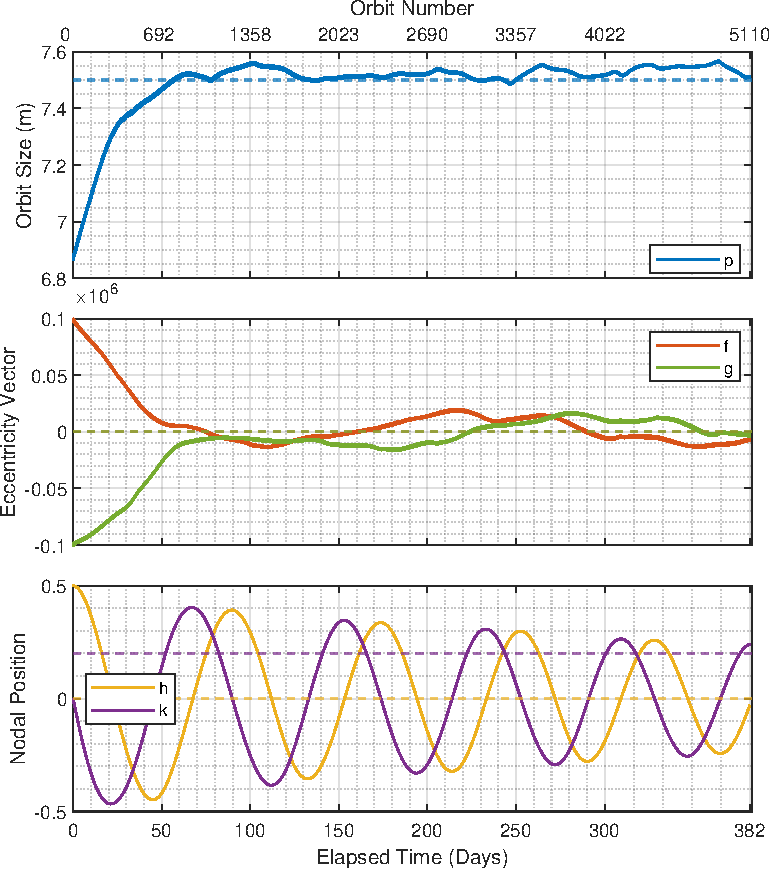
\includegraphics[width=\textwidth]{figures/leo_operations/orbital_elements.pdf}
        \caption{Evolution of orbit elements in time.}
        \label{fig:results_results_j_a}
    \end{subfigure}
    \begin{subfigure}[t]{0.59\textwidth}
        \animategraphics[width=\textwidth, controls, loop]{10}{animations/leo_operations/anim-}{1}{51}
        \caption{Trajectory animation.}
        \label{fig:results_results_j_b}
    \end{subfigure}
    \caption{Orbital elements and trajectory for case J.}
    \label{fig:results_results_j}
\end{figure}
The effects of \(J2\) perturbation are clearly visible in the plots of \(h\) and \(k\). Despite the challenging conditions, QUAIL manages to perform the maneuver without issues.

It is interesting to note that the spacecraft performed over 5000 revolutions of Earth during its maneuver. This highlights the key advantage of using a feedback approach over a global method -- a global optimization approach would likely be computationally intractable for a case like this.

\section{Realistic Solar Sail Modelling Study}

Cases A and B were run with modified values of \(\kappa\), and with all other parameters kept the same as the baseline values. The impact on time of flight is shown in Table \ref{tab:cone_angle_changing}.

\begin{table}[H]
    \centering
    \begin{tabular}{ccc}
        \toprule
                   & \multicolumn{2}{c}{Time of Flight (d)}          \\
        \(\kappa\) & Case A                                 & Case B \\
        \midrule
        \ang{90}   & 1410                                   & 555    \\
        \ang{80}   & 1136                                   & 544    \\
        \ang{70}   & 941                                    & 515    \\
        \ang{60}   & 616                                    & 422    \\
        \ang{50}   & 1126                                   & 389    \\
        \ang{40}   & 1528                                   & 395    \\
        \ang{30}   & 2097                                   &        \\
        \ang{20}   &                                        &        \\
        \ang{10}   &                                        &        \\
        \bottomrule
    \end{tabular}
    \caption{Variation of time of flight against an artificially restricted value of \(\kappa\). Blank entries denote no convergence.}
    \label{tab:cone_angle_changing}
\end{table}

There is a clear optimum for \(\kappa\), which is reasonable; that value represents the best tradeoff between producing thrust in the desired direction, and producing a sufficiently great amount of thrust.

It is surprising that transfers are still working even with \(\kappa = \ang{40}\). This is a testament to the robustness of the Q-Law against plant dynamics variation, and suggests that QUAIL may work quite well even with very restrictive cone angle limits.

It is also reassuring to see that the guidance law has limits to its capabilities; it for an extremely restrictive thrust cone angle, it simply cannot produce thrust in the direction needed by the Q-Law for progress towards the target orbit.

\section{Discussion}
While QUAIL demonstrates great success in all of the numerical experiments, the methodology must be scrutinized to assess the validity of the claims being made.

The lack of theoretical performance guarantees means that QUAIL can only be assessed through exhaustive simulation testing. In this thesis, only a handful of cases were simulated, and although they are challenging, they do not encompass the entire range of possible orbital maneuvers which may be done with a real solar sail. The issues encountered with the GEO disposal case raise concern over the performance of the guidance law with more ``benign'' orbital transfer cases, which may not have been captured by the other 3 cases. For future work, a better set of baseline cases should be developed, including a variety of cases motivated by practical maneuvers (de-orbiting, maneuvering to scientifically valuable orbits, etc.) rather than just trying to change many orbital elements all at once. \textbf{Both the quantity and quality of the trajectory cases should be improved} for future work. Nonetheless, the observed performance seen in the preceding experiments strongly suggests that QUAIL is able to perform complex orbital transfers.

The guidance optimization study is quite well done, and shows that improvement in performance is possible. However, no general trends or heuristics on how to tune the guidance law are developed, as there are only 2 cases which were optimized. An interesting study would be to develop a tuning heuristic for QUAIL which can be applied \textit{a priori} or with fewer simulation runs, somewhat like Ziegler-Nichols PID tuning \cite{ziegler1942optimum}.

For disturbance rejection analysis, while \(J2\) perturbations are dominant in low Earth orbit, most solar sails operate in higher orbits where these effects are not as significant. It would be more interesting to investigate gravitational perturbations from the Sun and Moon, or atmospheric drag effects. It is also difficult to justify claims about QUAIL's performance given that only a single case was run.

The realistic solar sail modelling study is quite limited in its scope and usefulness. An improved study with an actual thrust model featuring off axis thrust may reveal more subtle features of working with solar sails that is not available with using an ideal sail thrust model.

Additionally, attitude dynamics have not been considered. For sufficiently long period orbits, this should not have a great effect on performance, but it would be desirable to test QUAIL in a simulator with limits imposed on the angular rates of the spacecraft.

Overall, the few experiments which were conducted with QUAIL cannot be used to certify performance, but suggest that even with further testing, QUAIL can prove to be a very reliable and performant guidance law for solar sailing.